%************************************************
\chapter{User Guide}\label{ch:user_guide} % $\mathbb{ZNR}$
%************************************************

In this chapter an overview over the possible use-cases a user can accomplish will be provided, including pictured tutorials about how to achieve a use case.

The described use cases are:

\begin{itemize}
\item Login (and registering).
\item Searching for products.
\item Adding items to the shopping cart.
\item Editing items in the shopping cart.
\end{itemize}

\section{Login (and registering)}
\label{sec:login}

When the page is loaded and the user is not yet logged in, a sidebar will provide the necessary form to allow the user to login:

\begin{figure}[H]
\begin{center}
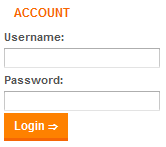
\includegraphics[scale=1]{gfx/login.png}
\caption{Login panel}
\label{fig:login}
\end{center}
\end{figure}

If the user does not yet have a login, he can either click on the \texttt{Register}-tab in the header or use the link provided in the homepage-text.

\begin{figure}[H]
\begin{center}

\includegraphics[scale=1]{gfx/header.png}
\caption{The header links}
\label{fig:header}
\end{center}
\end{figure}

This will open up the register website, where the user enter his details and create an account.
Should the entered details not fulfil the requirements (not entering the same password twice, entering no data in a field), the form will display the errors and urge the user to correct them:

\begin{figure}[H]
\begin{center}
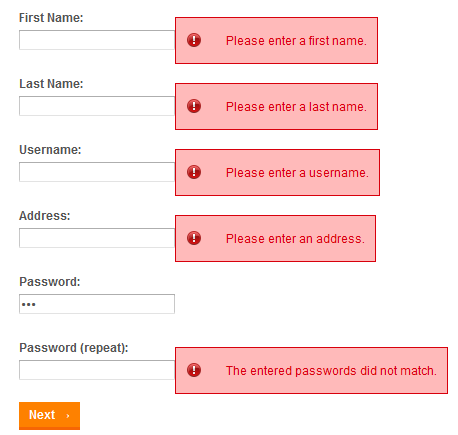
\includegraphics[scale=1]{gfx/login_errors.png}
\caption{The register form displays errors.}
\label{fig:register_errors}
\end{center}
\end{figure}

Should the user try to access a page without logging in first a redirection to the main page will occur and an information will be displayed:

\begin{figure}[H]
\begin{center}
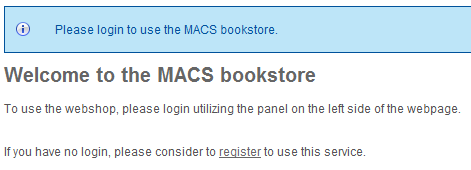
\includegraphics[scale=1]{gfx/access_denied.png}
\caption{Information to login first}
\label{fig:access_denied}
\end{center}
\end{figure}

\section{Searching for products}
\label{sec:searching}

After logging in the user can access the search page by clicking on the \texttt{Products} link in the header and the search page will be displayed.

On that page the user can check the category that shall be search, as well as provide a string that shall be searched:

\begin{figure}[H]
\begin{center}
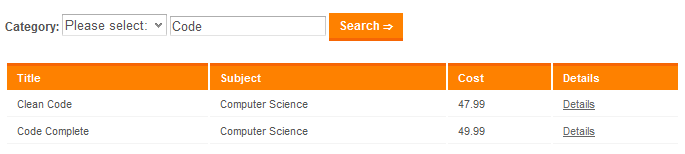
\includegraphics[width=\textwidth]{gfx/search.png}
\caption{Searching for products}
\label{fig:header}
\end{center}
\end{figure}

The possible categories are: \texttt{Title, Author, Publisher and Topic}. If the user does not select a category and attempts a search then all categories will be used to attempt a match.

If no search string is entered all available products will be displayed.

\section{Adding items to the shopping cart}
\label{sec:adding_items}

Items can be added from the details page of an item. To reach this page a click on the link in the search-results list is enough.

On the the details page the user can fill out a form that add the chosen number of products to the shopping cart:

\begin{figure}[H]
\begin{center}
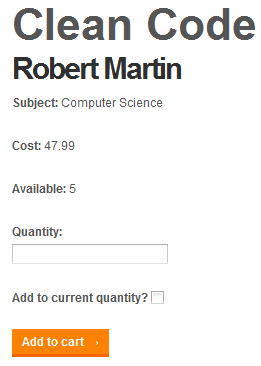
\includegraphics[scale=1]{gfx/add_product.png}
\caption{Adding a product to the shopping cart.}
\label{fig:add_product}
\end{center}
\end{figure}

When the product is successfully added to the shopping cart the website will display a message to confirm it:

\begin{figure}[H]
\begin{center}
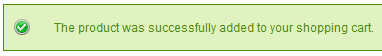
\includegraphics[scale=1]{gfx/adding_successful.png}
\caption{Product successfully added.}
\label{fig:successful_add}
\end{center}
\end{figure}

Should the user provide an incorrect number of products (e.g. none or not a number) the website will notify the user about the error.

\begin{figure}[H]
\begin{center}
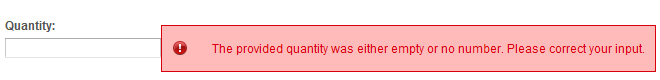
\includegraphics[width=\textwidth]{gfx/incorrect_quantity.png}
\caption{User is informed about incorrect input.}
\label{fig:incorrect_add}
\end{center}
\end{figure}


\section{Editing items in the shopping cart}
\label{sec:editin_items}

When the user clicks on the shopping cart link in the header, this will redirect him to the shopping cart. There all items will be displayed in a table and it is possible to remove items that are currently in the cart, as well as update the current quantity of items:

\begin{figure}[H]
\begin{center}
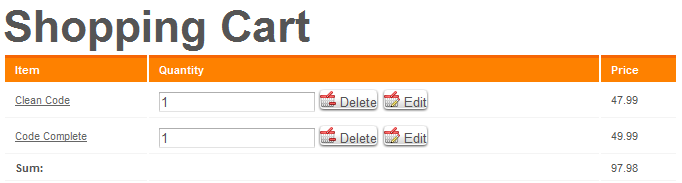
\includegraphics[width=\textwidth]{gfx/shopping_cart.png}
\caption{The shopping cart.}
\label{fig:shopping_cart}
\end{center}
\end{figure}

When the user clicks the \texttt{delete}-button (\raisebox{-1mm}{
\includegraphics{gfx/basket-minus.png}}) the item that is present in that table row will be removed from the shopping cart.

When the user enters a new quantity and clicks the \texttt{edit}-button (\raisebox{-1mm}{
\includegraphics{gfx/basket-pencil.png}}) the item's quantity will be updated to the one entered.

Should the user enter an illegal quantity, the web page will display an error and the operation will not be executed.

\begin{figure}[H]
\begin{center}
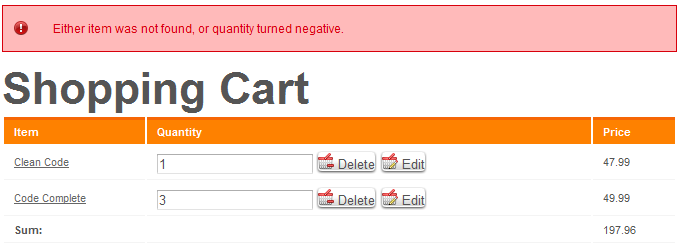
\includegraphics[width=\textwidth]{gfx/illegal_edit.png}
\caption{Illegal edit is prevented.}
\label{fig:illegal_edit}
\end{center}
\end{figure}